\chapter{مقدمة}
\label{ch:introduction}

% مقدمة تمهيدية للفصل
يُعد التحكم بالحركة (\textenglish{Motion Control}) أحد أهم الركائز التي تعتمد عليها أنظمة الأتمتة الصناعية الحديثة لضمان أداء دقيق وموثوق. يهدف هذا الفصل إلى وضع حجر الأساس النظري لفهم هذه المنظومات، حيث يستعرض المفاهيم الأساسية للتحكم الحركي، ويفصل المكونات الرئيسية التي تتألف منها، بالإضافة إلى تسليط الضوء على الفروقات الجوهرية بين أنظمة التحكم ذات الحلقة المفتوحة (\textenglish{Open-Loop}) وتلك ذات الحلقة المغلقة (\textenglish{Closed-Loop}). سيمهد هذا الاستعراض النظري الطريق للتعمق لاحقاً في التشريح الداخلي لمحركات السيرفو واستراتيجيات التحكم المتقدمة بها.

\vspace{0.5cm} % مسافة فاصلة قبل بدء الأقسام الفرعية

\section{تعريف النظام ومكوناته الأساسية}
\label{sec:components}

تُعرّف أنظمة التحكم بالحركة (\textenglish{Motion Control Systems}) بأنها أنظمة هندسية متكاملة تُعنى بالتحكم الدقيق والمستمر في المتغيرات الديناميكية للحركة، والتي تشمل الموضع (\textenglish{Position})، السرعة (\textenglish{Velocity})، والتسارع (\textenglish{Acceleration}). تلعب هذه الأنظمة دوراً محورياً في تطبيقات الأتمتة الصناعية الحديثة، حيث تضمن تنفيذ المناورات الحركية المعقدة بكفاءة وتكرارية عالية وثبات ديناميكي، لا سيما في الآلات ذات التحكم الرقمي (\textenglish{CNC}) والمنظومات الروبوتية المتقدمة.

% المخطط الصندوقي للمكونات
\begin{figure}[h!]
    \centering
    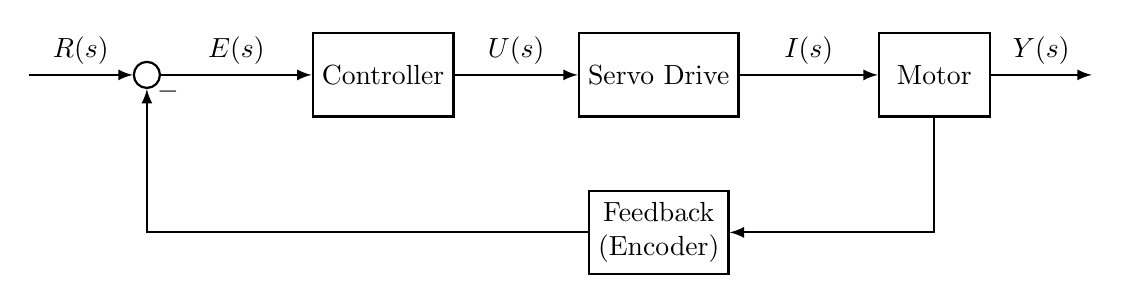
\begin{tikzpicture}[auto, node distance=2.5cm, >=latex]
        % تعريف أشكال الكتل
        \tikzstyle{block} = [draw, rectangle, minimum height=3em, minimum width=4em, align=center, thick]
        \tikzstyle{sum} = [draw, circle, node distance=1.5cm, thick]
        \tikzstyle{input} = [coordinate]
        \tikzstyle{output} = [coordinate]

        % رسم العقد (Nodes)
        \node [input] (ref) {};
        \node [sum, right of=ref] (sum) {};
        \node [block, right of=sum, node distance=3cm] (controller) {\textenglish{Controller}};
        \node [block, right of=controller, node distance=3.5cm] (drive) {\textenglish{Servo Drive}};
        \node [block, right of=drive, node distance=3.5cm] (motor) {\textenglish{Motor}};
        \node [output, right of=motor, node distance=2cm] (out) {};
        \node [block, below of=drive, node distance=2cm] (feedback) {\textenglish{Feedback}\\\textenglish{(Encoder)}};

        % رسم الأسهم والمسارات (Edges)
        \draw [->, thick] (ref) -- node [above] {$R(s)$} (sum);
        \draw [->, thick] (sum) -- node [above] {$E(s)$} (controller);
        \draw [->, thick] (controller) -- node [above] {$U(s)$} (drive);
        \draw [->, thick] (drive) -- node [above] {$I(s)$} (motor);
        \draw [->, thick] (motor) -- node [above] (y) {$Y(s)$} (out);
        \draw [->, thick] (motor) |- (feedback);
        \draw [->, thick] (feedback) -| node[pos=0.99, right] {$-$} (sum);
    \end{tikzpicture}
    \caption{\centering{مخطط صندوقي يوضح المكونات الأساسية لنظام التحكم بالحركة ذو الحلقة المغلقة}}
    \label{fig:motion_components}
\end{figure}

\subsection{مسار الإشارة والمكونات الفعالة}
كما يتبين من المخطط الصندوقي في الشكل (\ref{fig:motion_components})، يتكون نظام التحكم بالحركة الحلقي المغلق من أربعة عناصر أساسية تتفاعل ديناميكياً فيما بينها لضمان تتبع المسار المطلوب بدقة:

\begin{enumerate}
    \item \textbf{وحدة التحكم بالحركة (\textenglish{Motion Controller}):}
    تمثل العقل المدبر ومصدر القرار في النظام. تستقبل هذه الوحدة إشارة الخطأ $E(s)$ الناتجة عن مقارنة الدخل المرجعي $R(s)$ مع التغذية الراجعة. تتلخص وظيفتها في توليد وتخطيط مسار الحركة الزمني (\textenglish{Trajectory Generation})، ومن ثم إنتاج إشارة تحكم $U(s)$ بناءً على خوارزميات التحكم المطبقة (مثل \textenglish{PID}).
    
    \item \textbf{مُشغل القدرة أو المكبر (\textenglish{Servo Drive / Amplifier}):}
    يعمل كوسيط طاقة بين وحدة التحكم والمحرك. يستقبل المشغل إشارة التحكم القيادية $U(s)$، ويقوم بتضخيمها وتحويلها إلى كميات تيار وجهد ملائمة $I(s)$ لتوليد العزم المغناطيسي المطلوب في المحرك، مع مراعاة حماية النظام من التيارات الزائدة.
    
    \item \textbf{المُحرك (\textenglish{Actuator / Servo Motor}):}
    هو العضو التنفيذي المسؤول عن تحويل الطاقة الكهربائية القادمة من المشغل إلى طاقة ميكانيكية حركية $Y(s)$. تمتاز محركات السيرفو بالقدرة على تحمل أحمال متغيرة وتوفير تسارعات عالية بفضل انخفاض عزم القصور الذاتي لعضوها الدوار.
    
    \item \textbf{حساس التغذية الراجعة (\textenglish{Feedback Device}):}
    يمثل عين النظام التي تراقب الأداء في الوقت الحقيقي. يُثبت هذا الحساس (مثل المشفرات \textenglish{Encoders}) لقياس المخرج الفعلي $Y(s)$، وإرسال هذه القياسات عودةً إلى نقطة المقارنة لإغلاق حلقة التحكم وتصحيح أي انحراف عن المسار المستهدف بشكل مستمر.
\end{enumerate} % تعريف النظام ومكوناته
\section{أنظمة الحلقة المفتوحة مقابل الحلقة المغلقة}
\label{sec:open_closed_loop}

تُصنف أنظمة التحكم بالحركة في الأتمتة الصناعية بناءً على آلية معالجتها للإشارات وتصحيحها للأخطاء الديناميكية إلى صنفين رئيسيين: أنظمة الحلقة المفتوحة، وأنظمة الحلقة المغلقة. يكمن الفارق الجوهري بينهما في وجود أو غياب مسار التغذية الراجعة (\textenglish{Feedback Path}).

% المخططات الصندوقية للمقارنة
\begin{figure}[h!]
    \centering
    
    % --- عنوان المخطط الأول ---
    {\centering \textarabic{\textbf{(أ) نظام تحكم مفتوح الحلقة}} \\ \textenglish{\textbf{(Open-Loop)}} \\[0.5cm]}
    
    % --- رسم نظام الحلقة المفتوحة ---
    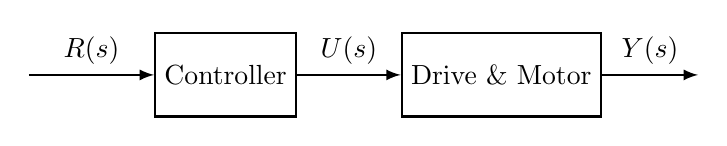
\begin{tikzpicture}[auto, node distance=2.5cm, >=latex]
        % تعريف الأنماط
        \tikzstyle{block} = [draw, rectangle, minimum height=3em, minimum width=4em, align=center, thick]
        \tikzstyle{input} = [coordinate]
        \tikzstyle{output} = [coordinate]

        \node [input] (ref_open) {};
        \node [block, right of=ref_open, node distance=2.5cm] (ctrl_open) {\textenglish{Controller}};
        \node [block, right of=ctrl_open, node distance=3.5cm] (plant_open) {\textenglish{Drive \& Motor}};
        \node [output, right of=plant_open, node distance=2.5cm] (out_open) {};

        \draw [->, thick] (ref_open) -- node [above] {$R(s)$} (ctrl_open);
        \draw [->, thick] (ctrl_open) -- node [above] {$U(s)$} (plant_open);
        \draw [->, thick] (plant_open) -- node [above] {$Y(s)$} (out_open);
    \end{tikzpicture}
    
    \vspace{1.5cm} % مسافة فاصلة بين المخططين
    
    % --- عنوان المخطط الثاني ---
    {\centering \textarabic{\textbf{(ب) نظام تحكم مغلق الحلقة}} \\ \textenglish{\textbf{(Closed-Loop)}} \\[0.5cm]}
    
    % --- رسم نظام الحلقة المغلقة ---
    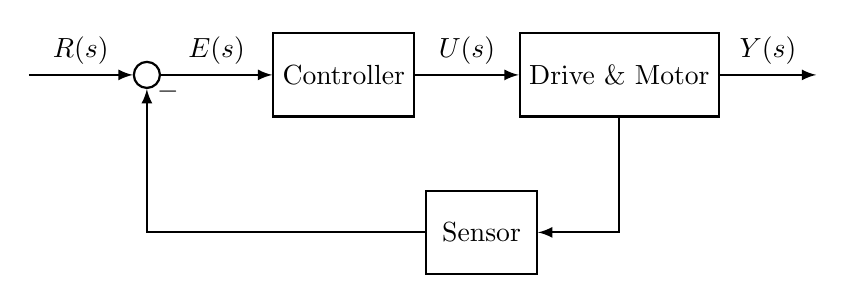
\begin{tikzpicture}[auto, node distance=2.5cm, >=latex]
        % تعريف الأنماط
        \tikzstyle{block} = [draw, rectangle, minimum height=3em, minimum width=4em, align=center, thick]
        \tikzstyle{sum} = [draw, circle, node distance=1.5cm, thick]
        \tikzstyle{input} = [coordinate]
        \tikzstyle{output} = [coordinate]

        \node [input] (ref_closed) {};
        \node [sum, right of=ref_closed, node distance=1.5cm] (sum_closed) {};
        \node [block, right of=sum_closed, node distance=2.5cm] (ctrl_closed) {\textenglish{Controller}};
        \node [block, right of=ctrl_closed, node distance=3.5cm] (plant_closed) {\textenglish{Drive \& Motor}};
        \node [output, right of=plant_closed, node distance=2.5cm] (out_closed) {};
        \node [block, below of=ctrl_closed, node distance=2cm, xshift=1.75cm] (fb_closed) {\textenglish{Sensor}};

        \draw [->, thick] (ref_closed) -- node [above] {$R(s)$} (sum_closed);
        \draw [->, thick] (sum_closed) -- node [above] {$E(s)$} (ctrl_closed);
        \draw [->, thick] (ctrl_closed) -- node [above] {$U(s)$} (plant_closed);
        \draw [->, thick] (plant_closed) -- node [above] (y_cl) {$Y(s)$} (out_closed);
        \draw [->, thick] (plant_closed) |- (fb_closed);
        \draw [->, thick] (fb_closed) -| node[pos=0.99, right] {$-$} (sum_closed);
    \end{tikzpicture}

    \caption{{\centering مقارنة هيكلية بين مسار الإشارة في أنظمة الحلقة المفتوحة والحلقة المغلقة}}
    \label{fig:open_vs_closed}
\end{figure}

\subsection{أنظمة الحلقة المفتوحة (\textenglish{Open-Loop Systems})}
في هذه الأنظمة، تُرسل وحدة التحكم أوامر الحركة (على شكل نبضات عادةً) إلى المشغل والمحرك دون التحقق من التنفيذ الفعلي للحركة، كما هو موضح في الشكل (\ref{fig:open_vs_closed}-أ). تُعد المحركات الخطوية (\textenglish{Stepper Motors}) التطبيق الأشهر لهذه الأنظمة.
\begin{itemize}
    \item \textbf{المزايا:} بساطة التصميم، انخفاض التكلفة، وسهولة البرمجة لعدم وجود خوارزميات معالجة للخطأ.
    \item \textbf{العيوب:} ضعف الاستجابة للديناميكيات المتغيرة، وخطر "فقدان الخطوات" (\textenglish{Loss of Steps}) عند تعرض المحرك لعزم تحميل يتجاوز قدرته، مما يؤدي إلى خطأ دائم في التموضع لا يمكن للنظام اكتشافه.
\end{itemize}

\subsection{أنظمة الحلقة المغلقة (\textenglish{Closed-Loop Systems})}
تعتمد هذه الأنظمة على مبدأ التغذية الراجعة المستمرة لتصحيح الخطأ الديناميكي $E(s)$، كما في الشكل (\ref{fig:open_vs_closed}-ب). تُعتبر محركات السيرفو (\textenglish{Servo Motors}) الممثل الرئيسي لهذا النوع. في التطبيقات الصناعية المتقدمة، تُقسم هذه الأنظمة إلى:
\begin{enumerate}
    \item \textbf{نظام حلقة شبه مغلقة (\textenglish{Semi-Closed Loop}):} يتم تثبيت حساس التغذية الراجعة (المشفر) على محور المحرك مباشرة. يُعد هذا النظام الأكثر شيوعاً، إلا أنه لا يكتشف الأخطاء الميكانيكية الناتجة عن الوصلات كالسماحية الميكانيكية (\textenglish{Backlash}) في صناديق التروس.
    \item \textbf{نظام حلقة مغلقة بالكامل (\textenglish{Fully Closed Loop}):} يتم تثبيت حساس إضافي (مثل مسطرة قياس خطية \textenglish{Linear Scale}) على الحمل الميكانيكي النهائي (كالطاولة المتحركة في آلات \textenglish{CNC}). يوفر هذا النظام أقصى درجات الدقة لأنه يعوض جميع الأخطاء الميكانيكية المتراكمة في سلسلة نقل الحركة.
\end{enumerate}

\subsection{جدول مقارنة شامل}
يلخص الجدول التالي (\ref{tab:comparison}) أبرز الفروقات الهندسية والتشغيلية بين الأنظمة الثلاثة، مما يبرز التدرج في الدقة والتعقيد:

\begin{table}[h!]
    \centering
    \renewcommand{\arraystretch}{1.4}
    \begin{tabular}{|p{3cm}|p{3.5cm}|p{4cm}|p{4cm}|}
        \hline
        \textbf{وجه المقارنة} & \textbf{الحلقة المفتوحة} & \textbf{الحلقة شبه المغلقة} & \textbf{الحلقة المغلقة بالكامل} \\
        \hline
        \textbf{مكان الحساس} & لا يوجد & على محور المحرك مباشرة & على الحمل الميكانيكي النهائي \\
        \hline
        \textbf{مستوى الدقة} & متوسطة (تتأثر بالأحمال وتفقد خطوات) & عالية (لكن لا تكتشف السماحية الميكانيكية \textenglish{Backlash}) & قصوى (تُعوض جميع الأخطاء الميكانيكية للوصلات) \\
        \hline
        \textbf{التعقيد والضبط} & بسيط (لا يتطلب ضبط \textenglish{Tuning}) & معقد (يتطلب ضبط معاملات \textenglish{PID}) & معقد جداً (احتمالية حدوث رنين ميكانيكي \textenglish{Resonance}) \\
        \hline
        \textbf{التكلفة} & اقتصادية جداً & مرتفعة & باهظة (تتطلب حساسات قياس إضافية عالية الدقة) \\
        \hline
    \end{tabular}
    \caption{{\centering مقارنة هندسية بين أنظمة الحركة المفتوحة، شبه المغلقة، والمغلقة بالكامل}}
    \label{tab:comparison}
\end{table} % مقارنة حلقات التحكم 